\documentclass[sigconf,nonacm]{acmart}
\usepackage{graphicx}
\usepackage{subcaption}
\usepackage{caption}
\captionsetup[subfigure]{skip=2pt}
\captionsetup[figure]{skip=4pt}
\usepackage{booktabs}
\usepackage{tabularx}
\usepackage{placeins}
\usepackage{xcolor}
\setlength{\emergencystretch}{2em}

\newcommand{\fillin}[1]{\textcolor{red}{[#1]}}
\newcommand{\eventphoto}[2]{%
  \IfFileExists{figures/photos/#1}{%
    \includegraphics[width=#2,height=0.62#2,keepaspectratio]{figures/photos/#1}}{%
    \fbox{\parbox[c][0.45#2][c]{0.95#2}{\centering\footnotesize Photo\\\texttt{\detokenize{#1}}}}}}

\settopmatter{printacmref=false}
\renewcommand\footnotetextcopyrightpermission[1]{}
\pagestyle{plain}

\begin{document}

\title{The 3rd Annual AI Symposium and 2026 AI Applications Hackathon: Event report}

\author{\textmd{Authors (in alphabetical order):} \mbox{Gregory Blike}, \mbox{Nyingi Hannah Brown}, \mbox{Olivier Francois}, \mbox{Ajanee Igharo}, \mbox{Rebaz Kamal}, \mbox{Zhen Lu}, \mbox{Inal Mashukov}, \mbox{Rami Huu Nguyen}, \mbox{Viviana Romero-Alarcon}, \mbox{Moumita Saha}, \mbox{Balaji Tanniru}, \mbox{Chengjie Zheng}}
\author{\textmd{Editors:} \mbox{Viviana Romero-Alarcon}, \mbox{Rebaz Kamal}, \mbox{Balaji Tanniru}, \mbox{Rami Huu Nguyen}}
\affiliation{%
  \institution{Paul English Applied Artificial Intelligence Institute (PEAAII), University of Massachusetts Boston}
  \city{Boston}
  \state{Massachusetts}
  \country{USA}}

\renewcommand{\shortauthors}{PEAAII Student Advisory Council}

% ===============================================================
\begin{abstract}
The Paul English Applied Artificial Intelligence Institute (PEAAII) at UMass Boston hosted the 3rd Annual AI Symposium and the final round of the 2026 AI Applications Hackathon on October 29th 2026. The event was organized by the Student Advisory Council and the AI Symposium Organization Committee under the leadership of Professor Wei Ding, Executive Director of PEAAII, and aligned with her 'AI for All' vision. Attendees included Paul English, Provost Joseph Berger, Chief Information Officer David Albrecht, faculty, and industry representatives. The organizing team ensured free livestreaming and recording, facilitated student pitches, coordinated six final demo presentations, managed People's Choice voting and the awards ceremony, and invited student presenters from diverse majors to showcase their applied AI work. This structure provided students with a meaningful opportunity to present their projects to an audience of industry professionals and faculty. The event received 132 registration responses from students, staff, faculty, and guests; 88 in-person attendees; and 1,300 People's Choice votes cast online during the week before the final. More than 40 teams applied to the hackathon; 33 submitted projects and one later withdrew, leaving 32 projects spanning health and wellness, education, finance, workplace productivity, community services, travel, research and AI infrastructure. This report provides a comprehensive account of the organizing team's efforts, participant engagement, project outcomes, and recommendations for broadening disciplinary involvement and fostering future collaboration.

\end{abstract}

\keywords{Applied AI, hackathon, student leadership, AI education, event report, UMass Boston}

\maketitle

% ===============================================================
\section{Introduction}
PEAAII advances applied AI education and research at UMass Boston. Each fall, the institute organizes an AI Symposium that convenes students, faculty, staff, advisors, and industry partners to explore AI applications across the university and recognize student innovation. The 2026 third annual symposium featured the final showcase of the AI Applications Hackathon. To prepare the teams, the institute also ran the Applied AI Micro-credential, a series of workshops, and AI Demo Days on October 5th, 13th and 19th 2026, from 1:30 to 3:30 p.m.

Students played a central role in the planning and execution of the symposium. Under the direction of the Institute's Executive Leadership, the Student Advisory Council and the AI Symposium Organization Committee established multiple working groups to oversee venue and audiovisual arrangements, catering, outreach, registration, photography, and program delivery. These groups also managed hackathon presentations, judging, People’s Choice voting, and the awards ceremony. This report documents their collective contributions, recognizes the coordination necessary for the event's success, and serves as a resource for future organizers.

% ===============================================================
\section{Purpose and Goals}
The leadership team set the following goals for the event:
\begin{enumerate}
  \item \textbf{Showcase student innovation.} Give selected hackathon teams a public stage, including mature projects and early ideas with promise. Give finalists time for full live demonstrations.
  \item \textbf{Connect students with leaders.} Create direct contact between students and university leadership (the Provost and the CIO), the institute's namesake Paul English, faculty, advisors and industry guests.
  \item \textbf{Make AI accessible to all disciplines (``AI for All'').} Welcome participants from outside computer science through the essay contest, the AI for All session and a People's Choice vote that needs no technical background.
  \item \textbf{Recognize achievement.} Run a transparent awards process with judged and special-category prizes, a People's Choice prize for which teams publicize their own work and gather public votes, and participation awards for every team and essay.
  \item \textbf{Grow attendance.} Attract a larger and broader audience of students, faculty, staff and guests.
  \item \textbf{Document and share.} Capture the event through a professional photographer, a recorded livestream and written records for future organizing teams.
\end{enumerate}

% ===============================================================

\section{Event Overview}
The symposium took place on Thursday, October 29th 2026, from 10:00 a.m. to 4:00 p.m. in the Campus Center Ballrooms A-C. The room had a 24' x 12' stage, armchairs for the fireside chat, a judges' table, buffet tables, and room for approximately 150 people. University AV Services provided free live streaming and recording of the event on YouTube. Table \ref{tab:program} shows the program that was circulated to the community.


\begin{table}[t]
  \caption{Published program, October 29th 2026.}
  \label{tab:program}
  \small
  \begin{tabularx}{\columnwidth}{@{}lX@{}}
    \toprule
    \textbf{Time} & \textbf{Segment} \\
    \midrule
    10:00--10:30 & Photo session and registration \\
    10:30--10:42 & SAC Leadership Team on stage \\
    10:42--10:45 & Opening remarks, Provost Joseph Berger \\
    10:45--11:30 & Fireside chat: Paul English and Provost Berger, moderated by Wei Ding \\
    11:30--12:00 & AI for All student activities \\
    12:00--1:00  & Networking lunch and AI Innovation Showcase; leadership lunch \\
    1:00--2:10   & Hackathon lightning pitch competition \\
    2:10--3:20   & Hackathon final: six teams, live demos and judges' Q\&A \\
    3:20--3:30   & Judges' deliberation \\
    3:30--4:00   & Awards and recognition ceremony \\
    \bottomrule
  \end{tabularx}
\end{table}

\subsection{Preparation: workshops and AI Demo Days}
\label{sec:workshops}
The AI Demo Day Workshop Series (as part of the Applied AI Micro-credential Program) was all about preparing the students for the hackathon. The Demo Days took place on October 5th, 13th and 19th 2026, from 1:30 to 3:30 p.m.

On October 5th, Olivier Francois (Founder \& Researcher at WebAIAgent) kicked off with a hands-on session using Next.js, VS Code, and Cursor. Students explored how the parts of an AI agent work together (UI, LLM, agent logic, tools, application flow) using Olivier's working agent template and were encouraged to connect this to their own hackathon projects. The goal was to give students a grounding in how an AI agent application works rather than just having AI generate code. The session was accessible to students from all backgrounds regardless of their experience in agent development. Olivier Francois led the second Demo Day on October 13th. On October 19th, Inal Mashukov gave the talk "Stubborn and Hallucinating Agents: The Bias and Variance."

On October 9th, Amrita Datta (Global Marketing Strategist, Enterprise AI Advisor, VP and Board Member of AMA Boston) was a guest speaker in Professor Wei Ding's Industry AI Applications course. She gave a talk on her Global to Local (G2L) framework for adapting AI applications to different users and communities and on the five elements of trustworthy AI (guardrails, data boundaries, human in the loop, failure handling and evaluation). The students then applied these concepts to their hackathon projects in order to improve the security, reliability and user trust of their applications.

On October 23rd the Micro-credential students met with their AI advisors for feedback prior to the October 25th submission deadline (Section~\ref{sec:projects}). Slides from the October 5th and 9th sessions are available on UMass Boston ScholarWorks. Figure~\ref{fig:workshops} shows the workshops.

To support development, PEAAII bought \$217.87 worth of API credits for the hackathon teams to build and test their projects. The teams used \$38.19 of that (17.5\%), made around 16,800 API calls and processed around 626 million tokens. As 93.8\% of the requests were served from cache the average cost was around \$0.06 per million tokens so we were well within budget.

\begin{figure}[t]
  \centering
  \begin{subfigure}[t]{0.49\columnwidth}\centering
    \eventphoto{workshop_olivier_demo_day.jpg}{\linewidth}
    \caption{AI Demo Day led by Olivier Francois.}
  \end{subfigure}\hfill
  \begin{subfigure}[t]{0.49\columnwidth}\centering
    \eventphoto{workshop_inal_demo_day.jpg}{\linewidth}
    \caption{AI Demo Day with Inal Mashukov, October~19th.}
  \end{subfigure}\\[4pt]
  \begin{subfigure}[t]{0.49\columnwidth}\centering
    \eventphoto{ai_social_mixer.jpg}{\linewidth}
    \caption{AI Social Mixer led by Ajanee Igharo and Gregory Blike, October~20th.}
    \label{fig:mixer}
  \end{subfigure}
  \caption{Workshops, AI Demo Days and the AI Social Mixer before the symposium.}
  \label{fig:workshops}
\end{figure}

% ===============================================================
\section{Event Leadership}
The student leadership team set up the symposium as a space for education, sharing and celebration. The event organizers held weekly planning sessions to scope the event, assign tasks, and work with campus units to secure the venue, catering, registration and AV support. Janette White, Executive Assistant to the Provost, booked the Campus Center Ballrooms and arranged the initial AV support; building on her work, Ajanee Igharo secured strong support from AV Services, including the no-cost livestream. Adam Wise, Vice Chancellor of University Advancement, asked Virginia Paluzzi, Executive Assistant to the Vice Chancellor and University Advancement Office Director, to arrange catering for the entire symposium day and the SAC leadership lunch. Table~\ref{tab:leadership} in Appendix~\ref{app:leadership} details the roles and key contributions of each leader.

The team led outreach before and during the symposium for the Applied AI Micro-credential, the prep lab series and the AI Demo Days. Campus announcements, email and social media campaigns, and printed materials explained how students could participate and prepare. On September 23rd 2026, the SAC hosted a webinar to promote the Applied AI Micro-credential program; the recording was shared with students on UMass Boston's Canvas. On October 20th 2026, as one of the activities leading up to the hackathon, Ajanee Igharo and Gregory Blike also organized an AI Social Mixer to promote the program (Figure~\ref{fig:mixer}). Between September~1st and November~6th 2026, the team's LinkedIn posts about the symposium earned 14,790 impressions and 192 reactions. Managing registration, name-tag printing and participant communication helped welcome students, faculty, staff and external visitors.

This student leadership team created a shared run of show, assembled presentation slides, communicated speaking order and arrival times, and ran program and technical rehearsals to ensure a well-managed, coherent program. On the event day, emcees, timekeepers and presentation support kept the program on track and helped teams deliver their ideas and show their prototypes.

The organizers also created opportunities for engagement outside the competition. The fireside chat, AI for All program, networking lunch and innovation showcase connected students with university administrators, faculty, mentors and community guests. Judging, public People's Choice voting and the awards ceremony recognized student accomplishments, and the essay contest offered a forum for reflecting on artificial intelligence.

Finally, the team documented the event closely. The organizers wrote a photography plan and shot list, organized group photographs and recorded the program. Along with this report, these records document the event and will guide future organizers. Figure~\ref{fig:photos} shows the participant group, the SAC group and the award presentations.

\begin{table}[t]
  \caption{Event results.}
  \label{tab:kpi}
  \small
  \begin{tabularx}{\columnwidth}{@{}Xl@{}}
    \toprule
    \textbf{Measure} & \textbf{Result} \\
    \midrule
    Registration responses & 132 \\
    In-person attendance (peak headcount) & 88 \\
    LinkedIn impressions (September 1st--November 6th 2026) & 14,790 \\
    LinkedIn reactions (September 1st--November 6th 2026) & 192 \\
    API credits purchased for teams & \$217.87 \\
    API credits used by teams & \$38.19 (17.5\%) \\
    API usage by teams: requests / tokens & 16.8K / 626M \\
    Hackathon team applications & More than 40 \\
    Teams that submitted projects & 33 \\
    Teams withdrawn after submission & 1 \\
    Projects in competition & 32 \\
    Finalists with live demo & 6 \\
    Essay submissions & 30 \\
    Essays selected for ScholarWorks & 18 \\
    Livestream and recording & Yes, at no cost \\
    People's Choice votes (online, week before the final) & 1,300 \\
    Program ran on schedule & Yes \\
    \bottomrule
  \end{tabularx}
\end{table}

% ===============================================================
\section{Results}
The symposium brought together 88 in-person attendees, counted at the busiest point of the day; attendees checked in through self-registration. Separately, the People's Choice vote, open online during the week before the event, received 1,300 votes. The program ran on schedule from the opening remarks through the awards ceremony. Table~\ref{tab:kpi} summarizes the recorded outcomes.

University leadership and industry engagement supported direct interaction with students throughout the event. The Provost delivered opening remarks, participated in the fireside chat and served on the judging panel. Paul English and CIO David Albrecht also joined the judging panel and stayed throughout the event to hear students' perspectives.


% ===============================================================

\subsection{Registration and disciplinary reach}

The registration form received 132 responses between October 16th and October 29th 2026. Of these, 122 (92.4\%) came from people affiliated with UMass Boston and 10 (7.6\%) from people outside the university. These figures count registration responses, so they measure interest in the event rather than attendance; 88 people attended in person. Undergraduates made up 44\% of responses, PhD students 23\%, master's students 11\% and staff 8.3\% (11 responses); faculty and other affiliated roles accounted for the remaining 8 responses (6.1\%). Figure~\ref{fig:role} shows all roles.

\begin{figure}[t]
  \centering
  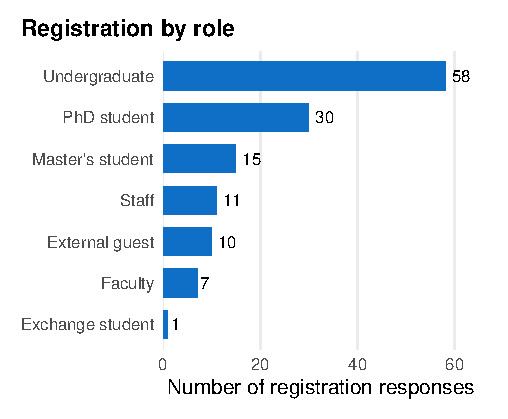
\includegraphics[width=\columnwidth]{figures/registration_by_role.pdf}
  \Description{}
  \caption{Registration by role: all 132 registration responses, including 11 staff and 10 guest responses.}
  \label{fig:role}
\end{figure}


Figure~\ref{fig:heatmap} breaks down the 111 responses from non-staff UMass Boston affiliates (students and faculty in a college or school) by role and by college or school. Staff responses (11) and responses from outside the university (10) are excluded. College groupings follow each registrant's reported program, with placements confirmed by the organizers. McCormack is included in Liberal Arts and Gerontology in Manning Nursing and Health Sciences.

%\clearpage
\begin{figure*}[t]
  \centering
  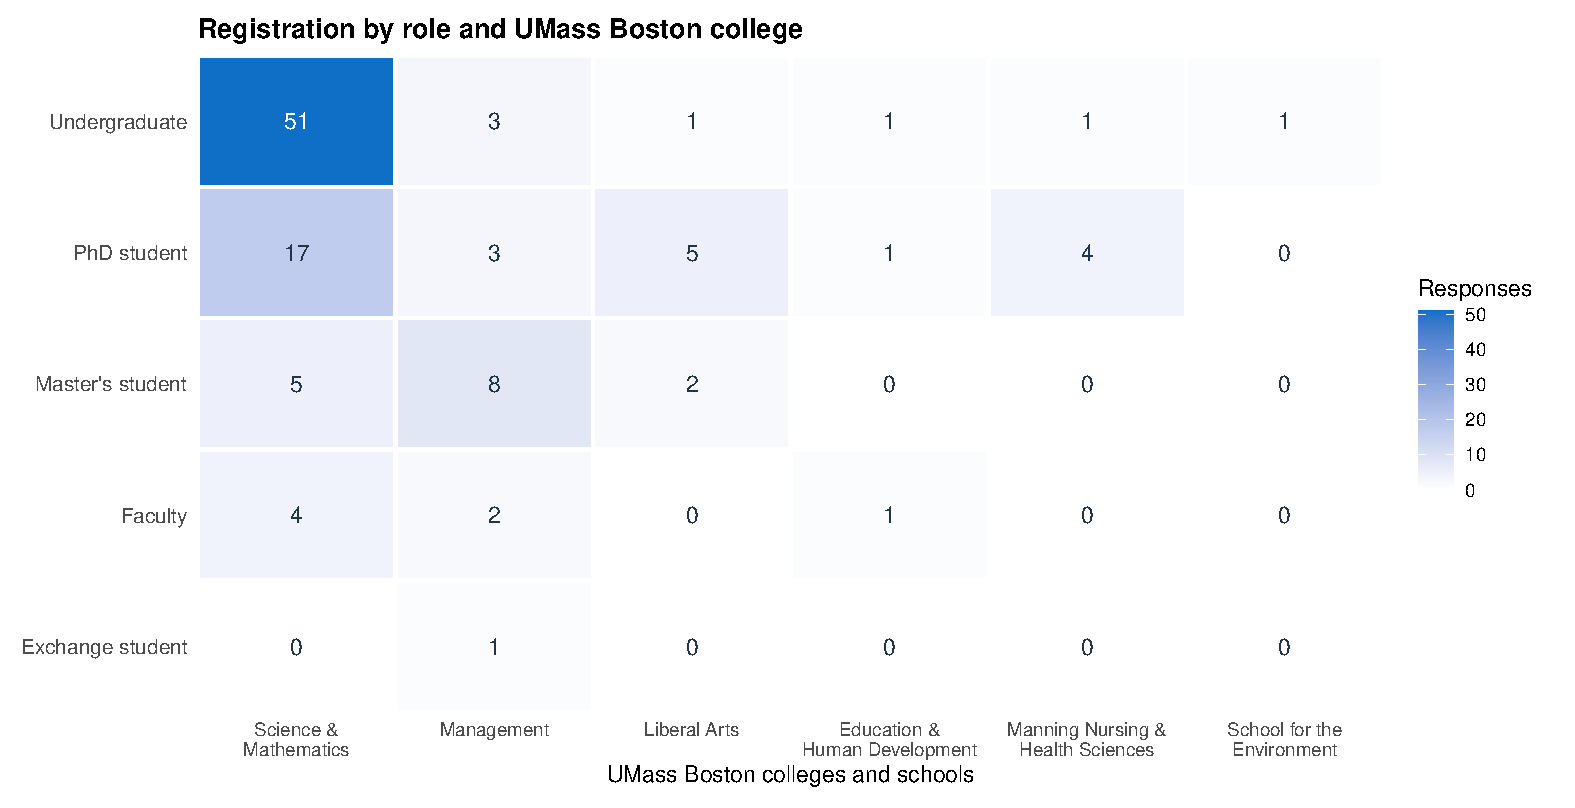
\includegraphics[width=\textwidth]{figures/registration_role_college_heatmap.pdf}
  \caption{Registration by role and UMass Boston college or school: 111 responses from affiliated students and faculty. Each cell shows registration responses; darker blue indicates more responses. Staff and outside-university registrations are excluded from this heatmap and reported separately in the text. College groups use program mappings and organizer confirmations; repeated registrations are retained.}
  \label{fig:heatmap}
\end{figure*}

As the heatmap shows, most responses came from the College of Science and Mathematics (77 of 111; 69.4\%), followed by the College of Management (17; 15.3\%). Smaller numbers came from Liberal Arts (8), Manning Nursing and Health Sciences (5), Education and Human Development (3) and the School for the Environment (1). This concentration points to an opportunity next year: targeted engagement to reach other colleges more broadly.

% ===============================================================

\subsection{Student projects and contest participation}
\label{sec:projects}

More than 40 teams applied to the hackathon. Thirty-three teams submitted projects, and one team later withdrew, leaving 32 projects in the competition. Six AI advisors from industry and the university helped choose the finalists (Table~\ref{tab:advisors} in Appendix~\ref{app:advisors}). On October~23rd, all students in the Applied AI Micro-credential Program were invited to meet with the advisors, who gave the hackathon teams feedback ahead of the October~25th submission deadline. The advisors then submitted their recommendations to Professor Wei Ding, Executive Director of PEAAII. Together, the advisors and Professor Ding selected six finalists from the 32 submissions based on intellectual merit and broader impacts: BlastBridge, ITDR, JustInCase, LiveTracker, Roameo and Signum. All 32 submissions are profiled in Appendix~\ref{app:profiles}. Across the submitted projects, the main application domains were health and wellness, education, finance, workplace productivity, community services, travel, research and AI infrastructure. Figure~\ref{fig:topics} shows the projects by primary topic. This range of topics shows the value of a public space where students from many disciplines can create, share and apply AI.

\begin{figure*}[t]
  \centering
  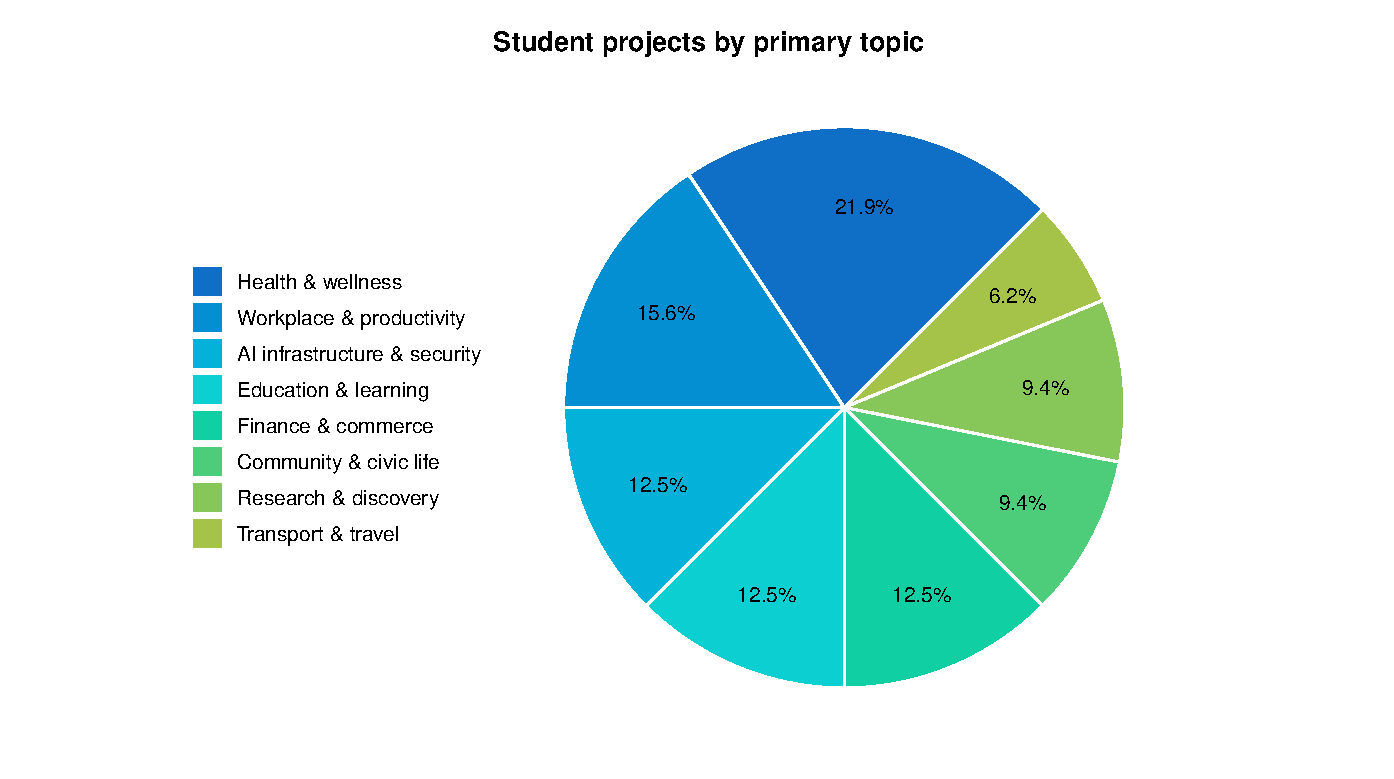
\includegraphics[width=0.94\textwidth]{figures/project_topics.pdf}
  \caption{Student projects by primary topic. Each project is assigned one primary topic; percentages use the 32 projects in the competition.}
  \label{fig:topics}
\end{figure*}

The essay contest offered another avenue for students who did not code. Thirty essays were submitted, all received recognition awards, and 18 were selected for publication in ScholarWorks. Together, the hackathon and the essay contest gave students two complementary venues: one for building applied AI projects and one for reflecting on the social, political and technical implications of AI.

% ===============================================================

\begin{figure*}[t]
  \centering
  \begin{subfigure}[t]{0.32\textwidth}\centering
    \eventphoto{all_participants.jpg}{\linewidth}
    \caption{All participants of the 3rd Annual AI Symposium.}
  \end{subfigure}\hfill
  \begin{subfigure}[t]{0.32\textwidth}\centering
    \eventphoto{all_participants_2.jpg}{\linewidth}
    \caption{Mixer and teams preparation for the Showcase.}
  \end{subfigure}\hfill
  \begin{subfigure}[t]{0.32\textwidth}\centering
    \eventphoto{sac_student_group.jpg}{\linewidth}
    \caption{The Student Advisory Council (SAC) with Executive Director Wei Ding, Paul English and CIO David Albrecht.}
  \end{subfigure}\\[4pt]
  \begin{subfigure}[t]{0.32\textwidth}\centering
    \eventphoto{award_first_prize.jpg}{\linewidth}
    \caption{First Prize.}
  \end{subfigure}\hfill
  \begin{subfigure}[t]{0.32\textwidth}\centering
    \eventphoto{award_second_prize.jpg}{\linewidth}
    \caption{Second Prize.}
  \end{subfigure}\hfill
  \begin{subfigure}[t]{0.32\textwidth}\centering
    \eventphoto{award_third_prize.jpg}{\linewidth}
    \caption{Third Prize.}
  \end{subfigure}\\[4pt]
  \begin{subfigure}[t]{0.32\textwidth}\centering
    \eventphoto{award_essay_prize.jpg}{\linewidth}
    \caption{AI Essay Contest winners.}
  \end{subfigure}\hfill
  \begin{subfigure}[t]{0.32\textwidth}\centering
    \eventphoto{award_multidisciplinary_prize.jpg}{\linewidth}
    \caption{Best Interdisciplinary Collaboration prize.}
  \end{subfigure}\hfill
  \begin{subfigure}[t]{0.32\textwidth}\centering
    \eventphoto{award_social_media_prize.jpg}{\linewidth}
    \caption{Social media voting (People's Choice) prize: Sync.}
  \end{subfigure}
  \caption{Photographic record of the symposium: the participant group photos, the SAC group and the six award presentations.}
  \label{fig:photos}
\end{figure*}

% ===============================================================


\begin{table}[t]
  \caption{Award structure and recipients.}
  \label{tab:awards}
  \small
  \begin{tabularx}{\columnwidth}{@{}Xrp{2.1cm}@{}}
    \toprule
    \textbf{Award} & \textbf{Amount} & \textbf{Recipient} \\
    \midrule
    First Place & \$3,500 & LiveTracker \\
    Second Place & \$2,500 & JustInCase \\
    Third Place & \$1,500 & Roameo \\
    Best Interdisciplinary Collaboration & \$1,500 & HistorAI \\
    AI for Social Good & \$1,500 & HealthBot \\
    People's Choice & \$1,500 & Sync \\
    Honorable Mention (3) & \$500 each & BlastBridge; ITDR; Signum \\
    Team Participation (33 teams) & \$100 each & All teams \\
    AI Essay Recognition (30) & \$50 each & Essay authors \\
    \midrule
    \textbf{Total awarded} & \textbf{\$18,300} & \\
    \bottomrule
  \end{tabularx}
\end{table}

\section{Awards}
The awards program recognized technical achievement, interdisciplinary collaboration, social impact and audience engagement. The six finalists gave live demonstrations and answered the judges' questions during the hackathon final (2:10--3:20~p.m.). The judging panel (Provost Joseph Berger, Paul English and CIO David Albrecht) then deliberated (3:20--3:30~p.m.). The panel selected the top three projects, the honorable mentions and the special-category recipients. The People's Choice Award was decided by a public online vote held during the week before the final. The organizers created a dedicated Microsoft Form for the vote, allowing one vote per person. Teams shared the form on social media, mainly LinkedIn, explaining their projects and asking for votes. The form received 1,300 votes, all cast before the event day; these votes are separate from the LinkedIn reactions reported in Table~\ref{tab:kpi}.

Several members of the organizing team also competed in the hackathon: Kepler (Rebaz Kamal, Rami Huu Nguyen, Balaji Tanniru, Moumita Saha, Olivier Francois and Nyingi Hannah Brown), Roameo (Zhen Lu), ZINC (Viviana Romero-Alarcon) and EvidenceLens (Ajanee Igharo). To keep the competition fair, finalists were selected by the AI advisors and Professor Wei Ding, the judged awards were decided by the three judges, and the People's Choice Award was decided by public vote. None of the judges or advisors belonged to a competing team.

LiveTracker received First Place, JustInCase Second Place, and Roameo Third Place. HistorAI earned Best Interdisciplinary Collaboration, HealthBot received AI for Social Good, and Sync won People's Choice. BlastBridge, ITDR and Signum received Honorable Mentions.

In addition, each of the 33 teams that submitted a project received a \$100 participation award, and 30 essay authors received \$50 recognition awards. PEAAII funded the full prize pool of \$18,300. Table~\ref{tab:awards} summarizes the awards and recipients.


% ===============================================================
\section{Challenges}
\begin{itemize}
  \item \textbf{Narrow disciplinary reach.} Most affiliated registrations came from the College of Science and Mathematics (69.4\%), with few from Liberal Arts, Nursing and Health Sciences, Education and the Environment.
  \item \textbf{Incomplete participant records.} Many team members' majors and roles were not recorded, which limits how precisely interdisciplinary participation can be measured.
  \item \textbf{Team attrition.} More than 40 teams applied, 33 submitted projects and one withdrew after submission.
\end{itemize}

% ===============================================================
\section{Recommendations for the Next Symposium}
Building on the leadership team's achievements, the next symposium should broaden participation by opening outreach earlier, inviting students from a wider range of departments, and offering accessible entry points through workshops, essays and project demonstrations.

Outreach should specifically prioritize the colleges with lower registration counts shown in the heatmap. Working with their faculty advisors and student organizations, sharing college-specific invitations, and offering examples of AI applications relevant to liberal arts, education, nursing and health sciences, and the environment can help increase participation next year.

An early AI Social Mixer and sustained faculty/advisor connections would help students form teams with complementary expertise and carry projects beyond the competition. A concise participation guide, a poster showcase and wider recognition of promising projects would give more students opportunities to present and receive feedback. A short team profile collected at registration should record each member's major and role, with consent, so interdisciplinary participation can be measured consistently. Promoting the API credits earlier and showing teams how to use them would let more of the budget support project development. A self-registration QR check-in at the entrance would make it easier to count attendance throughout the day. A small additional prize chosen by the audience in the room, where attendees vote for their favorite project from the showcase, would complement the online People's Choice vote.

Continuing the successful leadership model of named segment owners, student emcees, shared presentation materials and documented contributions will help future organizers preserve what worked while expanding the symposium's educational value.

% ===============================================================
\section{Conclusions}

The Student Advisory Council and AI Symposium Organization Committee translated student leadership into visible educational outcomes: a full-day public showcase, direct access to university and industry leaders, recognition across several forms of achievement, and a recorded platform for sharing applied AI work. This year's registrations and projects reached a wider range of fields, roles and topics, supporting the institute's commitment to AI for All, although participation from colleges beyond Science and Mathematics still needs to be strengthened. We warmly congratulate Professor Wei Ding and Paul English, who represent PEAAII and supported and guided this event from its first planning meeting to the awards ceremony. The next edition can build on these achievements through earlier community engagement, intentional team formation and continued support for students as they develop their projects.

\section{Sources and Reproducibility}
The figures in this report come from the event's own records. Registration data were collected through a registration form built in Microsoft Forms~\cite{msforms} (October 16th--October 29th 2026); in-person attendance was counted at the busiest point of the day, with attendees checking in through self-registration. People's Choice votes were collected through a dedicated Microsoft Form~\cite{msforms} that allowed one vote per person. LinkedIn impressions and reactions were taken from LinkedIn post analytics, and API credit usage from the provider's usage records. Team, project and essay counts come from the hackathon and essay contest submission records. Plots were produced in R~\cite{rcore2026} with the \texttt{ggplot2} package~\cite{wickham2016ggplot2}. The authors used generative AI tools to review the report: OpenAI's GPT-6.1 Sol in Light effort mode~\cite{openai2026gpt61} and Anthropic's Claude Opus 5.5 at Medium effort~\cite{anthropic2026opus55} for review of format and for auditing consistency, and Grammarly~\cite{grammarly2026} for review of syntax. The authors reviewed all suggestions and take full responsibility for the content of this report.
\\
GitHub: \textit{[repository URL to be added]}.\\
Zenodo DOI: \textit{[DOI to be added]}.

\begin{acks}
We extend our deepest congratulations and gratitude to Professor Wei Ding, Executive Director of PEAAII, and Paul English, the institute's namesake. As representatives of PEAAII, they supported and guided this event at every stage, and their shared vision of ``AI for All'' gave students the stage, the mentors and the resources to succeed. We thank PEAAII for funding the prize pool and the API credits. We thank Provost Joseph Berger, Paul English and CIO David Albrecht for serving as judges and speakers. We thank Janette White, Executive Assistant to the Provost, for booking the ballroom and arranging AV support, and Adam Wise, Vice Chancellor of University Advancement, and Virginia Paluzzi, Executive Assistant to the Vice Chancellor and University Advancement Office Director, for arranging the catering for the symposium and the SAC leadership lunch. We also thank Karissa Chute, Jose Reyes and Campus Center Operations; John Jessoe and AV Services; Sodexo; Quinn Graphics; the event photographer Sam Song; the AI advisors Preet Mehta, Maria Vasilevsky, Justin Q.~Pham, Dr.~Linsey Pang, Dr.~Henry Lo and Amrita Datta, who also joined us as a guest speaker; the faculty mentors; and every student who presented, wrote, volunteered or voted.
\end{acks}

\begin{thebibliography}{6}

\bibitem{anthropic2026opus55}
Anthropic. 2026.
\newblock Claude Opus 5.5 [Large language model].
\newblock Released September 22, 2026. Retrieved November 14, 2026 from \url{https://www.anthropic.com/news/claude-opus-5-5}

\bibitem{grammarly2026}
Grammarly, Inc. 2026.
\newblock Grammarly [Writing assistant software].
\newblock Retrieved November 14, 2026 from \url{https://www.grammarly.com}

\bibitem{msforms}
Microsoft Corporation. 2026.
\newblock Microsoft Forms [Online survey software].
\newblock Retrieved November 14, 2026 from \url{https://forms.office.com}

\bibitem{openai2026gpt61}
OpenAI. 2026.
\newblock GPT-6.1 Sol [Large language model].
\newblock Retrieved November 14, 2026 from \url{https://openai.com/index/introducing-gpt-6-1-sol/}

\bibitem{rcore2026}
R Core Team. 2026.
\newblock \emph{R: A Language and Environment for Statistical Computing}.
\newblock R Foundation for Statistical Computing, Vienna, Austria.
\newblock \url{https://www.R-project.org/}

\bibitem{wickham2016ggplot2}
Hadley Wickham. 2016.
\newblock \emph{ggplot2: Elegant Graphics for Data Analysis}.
\newblock Springer-Verlag, New York.
\newblock \url{https://ggplot2.tidyverse.org}

\end{thebibliography}



\clearpage
\onecolumn
\appendix

\section{Supplementary Material}
\label{app:leadership}
Table~\ref{tab:leadership} summarizes the event leadership team’s roles and principal contributions to the symposium. It documents responsibilities across program coordination, facilities and audiovisual support, outreach, registration, student activities, hackathon preparation, judging, awards and event documentation. Together, these contributions show how the team’s coordinated work supported a successful student-led event.
\begin{table}[htbp]
  \centering
  \caption{Event leadership and principal contributions.}
  \label{tab:leadership}
  \small
  \begin{tabularx}{\textwidth}{@{}p{3.3cm}p{4.2cm}X@{}}
    \toprule
    \textbf{Name} & \textbf{Role} & \textbf{Principal contributions} \\
    \midrule
    Wei Ding & PEAAII Executive Director; Distinguished Professor of CS & Overall direction and budget; moderated the fireside chat; presented the SAC leadership team; led awards and digital certificates. \\
    Rami Huu Nguyen & SAC core member & Run of show; venue requests to Campus Center Operations; promotion graphics and name tags; hackathon communications; moderated the lightning pitches and finals. \\
    Ajanee Igharo & SAC core member & Facilities and AV planning with Campus Center Operations and AV Services, including the no-cost livestream; collected fireside-chat questions; co-led the AI Social Mixer to promote the Micro-credential. \\
    Chengjie Zheng & SAC core member & Catering; self-registration and QR check-in; name tags and table tents; parking passes; lunch slides; emceed the closing networking session; printed materials. \\
    Rebaz Kamal & SAC core member & Marketing and Canvas announcements; consolidated slides and schedules for 33 teams; People's Choice submission links; technical operator during pitches. \\
    Gregory Blike & SAC core member & Fireside-chat question collection; co-led the AI Social Mixer to promote the Micro-credential; AI for All session and lunch wrap-up (co-emcee). \\
    Nyingi Hannah Brown & SAC core member & Led the AI Essay Contest (30 submissions); designed Module~4 of the Micro-credential; co-emcee for AI for All; award posters. \\
    Moumita Saha & SAC core member & Judges' deliberation segment (co-emcee); timekeeper for pitches. \\
    Zhen Lu & Organization Committee & People's Choice voting form; award slides and award board design. \\
    Viviana Romero-Alarcon & Organization Committee & Photographer plan and photo session (emcee); day-of checklist and to-do tracking; rehearsal logistics; drafted and prepared this report. \\
    Balaji Tanniru & Organization Committee & Technical support and debugging for teams; drafted and prepared this report. \\
    Olivier Francois & Organization Committee & Designed and led a hands-on AI development workshop (Next.js, TypeScript, APIs, OpenAI) to prepare hackathon teams. \\
    Inal Mashukov & Organization Committee & Hosted the HackMassachusetts event at UMass Boston; presented ``Stubborn and Hallucinating Agents: The Bias and Variance'' at the October~19th AI Demo Day. \\
    \bottomrule
  \end{tabularx}

%\FloatBarrier

\end{table}

\clearpage
\section{AI Advisors}
\label{app:advisors}
Table~\ref{tab:advisors} lists the six AI advisors who gave feedback to the hackathon teams and recommended the finalists. Amrita Datta also gave a guest lecture on trustworthy AI.
\begin{table}[htbp]
  \centering
  \caption{AI advisors for the 2026 AI Applications Hackathon.}
  \label{tab:advisors}
  \small
  \begin{tabularx}{\textwidth}{@{}p{3.2cm}p{5.0cm}X@{}}
    \toprule
    \textbf{Advisor} & \textbf{Position} & \textbf{Expertise} \\
    \midrule
    Preet Mehta & Manager, Healthcare Analytics, EXL Service & Data engineering and data platforms; healthcare analytics; data foundations for machine learning. \\
    Maria Vasilevsky & Manager of Operations and Outreach, Venture Development Center, UMass Boston & Operations and process improvement; external partnerships; project management (PMP, CSM); entrepreneurial ecosystems. \\
    Justin Q. Pham & Head of Product \& Design, Enterprise AI, PIMCO & Enterprise AI products; responsible AI, evaluation and governance; product strategy; UMass Boston alumnus. \\
    Dr.\ Linsey Pang & Distinguished AI Research Scientist, PayPal & Machine learning research (PhD, University of Sydney); previously at Salesforce, Walmart Labs and eBay. \\
    Dr.\ Henry Lo & Chief Technology Officer, TF Cornerstone & Applied AI in real estate and financial services; former McKinsey \& Company; PhD in AI, UMass Boston. \\
    Amrita Datta & Global Marketing Strategist and Enterprise AI Advisor; Vice President and Board Member, AMA Boston & Trustworthy AI (G2L Framework); global marketing strategy; cybersecurity and AI. \\
    \bottomrule
  \end{tabularx}
\end{table}

\clearpage
\section{Project Profiles}
\label{app:profiles}
\begingroup
\setlength{\parindent}{0pt}
\setlength{\parskip}{5pt}
\renewcommand{\arraystretch}{1.15}

The following profiles list each project with a short summary and its team members.

\subsection*{AgenticOps}
Resolve repetitive service-desk tickets and escalate cases needing a human.\\
\textit{Team:} Divyansh Chaubey, Oanh Nguyen, Aquil Gonsalves, Vybhavi Bailore.

\subsection*{HistorAI}
Connect generations by turning older adults life stories into approved articles and podcasts.\\
\textit{Team:} Louis Beckand Verwee, Giuliano Di Croce, Philipp Gaenz, Mattia Mencarelli.

\subsection*{LearningPulse}
Help students learn from course materials and help professors identify learning gaps.\\
\textit{Team:} Haniya Adil, Peter Bucci, Swikritee Chuke, John Ferraz, Drashti Patel, Anya Tongprasith, Ashriya Tuladhar.

\subsection*{HealthBot}
Turn wearable health data into contextual wellness reports and reviewed triage insights.\\
\textit{Team:} Kevin Chen, Koushik Das, Everett Labrecque, Deron Smoot.

\subsection*{GhostClick}
Replay browser workflows locally and repair changed page elements with bounded AI assistance.\\
\textit{Team:} Avanith Kanamarlapudi, Kalysha Melendez Hernandez, Chelsea Nguyen, Kurt Sooknanan, Ana Maria Fahlbock, Ila Lama.

\subsection*{ClinicalTrialAI}
Translate clinical-trial protocols into coordinator-approved patient guidance.\\
\textit{Team:} Rakesh Borra, Namratha Indla, Suchith Raj Patchigolla.

\subsection*{Research2Market}
Connect scientific evidence, engineering calculations and market analysis in a feasibility report.\\
\textit{Team:} Ahmet Aldatmaz, Ashley Alexandra, Andrea Galan, Rabia Genc, Aurelia Clarissa Hananto, Adam Khazynarko Legopranowo, Risty Kristiani Lende Mere, Davina Wolfe.

\subsection*{CrucibleCast}
Transform unfamiliar source data into validated, queryable records.\\
\textit{Team:} Abdulmani Abu, Guy Bilguun, Donnedy Charles, Luis Irizarry, Thai Nguyen, Sebastian Palomino Jimenez, Matthew Perez, Brandon Siscoe.

\subsection*{JustInCase}
Help people living alone prepare practical plans for everyday disruptions and support needs.\\
\textit{Team:} Joan Arches, Leya Kurzhiparambil, Satoshi Nagae, Oluwaseyi Omisore.

\subsection*{Signum}
Turn public city signals into signed, expiring advisories for robotaxi fleets.\\
\textit{Team:} Misha Bari, Mridhul Sharma, Cherise Smith-Medeiros.

\subsection*{EyeCatcher}
Give players evidence-based feedback from recordings of their gameplay.\\
\textit{Team:} Deaven Hudtohan, David Le, Tri Huynh, Evan Yang.

\subsection*{Sync}
Connect menstrual-cycle records with conversational tracking and wellness support.\\
\textit{Team:} Raneem Abuhasen, Sophia Cherkaoui, Daria Dobrolinski, Tien Le, Kayla Nguyen, Hrishita Pandya, Valentina Zheng.

\subsection*{StudyFlowAI}
Convert academic deadlines into conflict-free study plans that students approve.\\
\textit{Team:} Krish Gopani, Surya Sudhamshu Paravataneni, Rishank Singh, Sankalp Vaish, Sumukh Veeramalla.

\subsection*{CivicRoute}
Help residents report civic issues and help municipalities triage and track complaints.\\
\textit{Team:} Ayaz Mohammed, Abbas Shaik.

\subsection*{LiveTracker}
Support behavioral research with approved monitoring rules and evidence-based investigation of animal behavior.\\
\textit{Team:} Nasser Al Thani, Niyazi Develi, Sadaf Hamidy, Nandini Jain, Syed Taswar Mahbub, Ava Sajjadi, Karla Schallies, Asya Sezgin, Igor Ten.

\subsection*{HealthInsurancePriceTransparency}
Make negotiated insurance rates and denial context accessible through grounded comparisons.\\
\textit{Team:} Anthony Gong, Thea Hird, Felipe Mahecha Ramirez, Imad Saidi, Robinson Sanchez, Edwin Sorto Rosales, Erik Williamson.

\subsection*{ZINC}
Offer adaptable weekly plans for strength, mobility, reasoning and relaxation in midlife and later life.\\
\textit{Team:} Kesline Diogene Jean Baptiste, Anagha Patil, Viviana Romero-Alarcon, Sohan Arigela.

\subsection*{Sidekick}
Turn meeting discussion into reviewed scheduling, tasks and follow-up actions.\\
\textit{Team:} Chinmaya Murthy, Lakshmi Pranathi Vutla.

\subsection*{CircuitMax}
Help learners scan, simulate and debug breadboard circuits.\\
\textit{Team:} Jimmie Burge, Karl Francois, Ace Gool, Eyob Kidus.

\subsection*{ITDR}
Assemble identity-alert evidence and draft containment steps for analyst review.\\
\textit{Team:} John Dixon, Joseph Singletary, Keyshawn E. Jeannot, Lynn Constant, Thalyta G. Andrade, Wil Khouri, David T. Bonczar.

\subsection*{BlastBridge}
Organize military occupational and exposure history into evidence that people can review.\\
\textit{Team:} Matthew Fitzgerald, Jeff Lincoln, Sam Derenzo.

\subsection*{AgentGauge}
Test the actions of AI agents and expose unsafe or incorrect behavior before deployment.\\
\textit{Team:} Allan Martinez, Rhuan Saragioto.

\subsection*{InvoiceReviewAI}
Help finance teams check invoices against rules and flag cases for review.\\
\textit{Team:} Naim Cheref, Andy Mei, Thanh Van Nguyen, Thanh Duy Quach, Ishaan Rangnekar, Vinh Trac.

\subsection*{BuyTheRumor}
Convert market chatter into validated research briefs under user-defined limits.\\
\textit{Team:} Erika Severino, Daniel Neagu.

\subsection*{Kepler}
Connect construction plans with field evidence and support reviewed decisions about deviations.\\
\textit{Team:} Rebaz Kamal, Rami Huu Nguyen, Balaji Tanniru, Moumita Saha, Olivier Francois, Nyingi Hannah Brown.

\subsection*{MoneyMindAI}
Help young adults understand expenses and build personalized budget plans.\\
\textit{Team:} Chinyere Azike, Eric De Carvalho, Valerie Mann, Eric Moschella, Vu Phan.

\subsection*{EventPilot}
Help people plan events within a defined budget.\\
\textit{Team:} Enock Okorno Ayiku Ayiku, Haley Wodarczyk, Eloghosa Osemwekha.

\subsection*{AgentGate}
Check proposed AI-agent actions and allow, block or escalate them before execution.\\
\textit{Team:} Agatsya Vijaybhai Patel, Vraj Pinakin Soni.

\subsection*{PRAIFitness}
Combine workout tracking and personalized fitness guidance in an AI-supported coaching platform.\\
\textit{Team:} Nirmit Raj Dholakia, Jeny Sherchan.

\subsection*{Virtuoso}
Help shoppers compare products against preferences and track items of interest.\\
\textit{Team:} Aariba Amin, Zoha Amin, Zunairah Amin.

\subsection*{Roameo}
Build travel plans with checked budgets and traveler approval.\\
\textit{Team:} Noctis Zhang, Zhen Lu, Zhen Luo.

\subsection*{EvidenceLens}
Challenge early drug-discovery hypotheses with source-grounded counterevidence.\\
\textit{Team:} Ajanee Igharo, David Gogicajev.

\endgroup
\end{document}